%%%%%%%%%%%%%%%%%%%%%%%%%%%%%%%%%%%%%%%%%%%%%%%%%%%%%%%%%%%%%%%%%%%%%%%%%%%%%%%%
%2345678901234567890123456789012345678901234567890123456789012345678901234567890
%        1         2         3         4         5         6         7         8

\documentclass[letterpaper, 10 pt, conference]{ieeeconf}  % Comment this line out if you need a4paper

%\documentclass[a4paper, 10pt, conference]{ieeeconf}      % Use this line for a4 paper

\IEEEoverridecommandlockouts                              % This command is only needed if 
                                                          % you want to use the \thanks command

\overrideIEEEmargins                                      % Needed to meet printer requirements.

% See the \addtolength command later in the file to balance the column lengths
% on the last page of the document

% The following packages can be found on http:\\www.ctan.org
\usepackage{graphics} % for pdf, bitmapped graphics files
%\usepackage{epsfig} % for postscript graphics files
%\usepackage{mathptmx} % assumes new font selection scheme installed
%\usepackage{times} % assumes new font selection scheme installed
\usepackage[pdftex]{graphicx}
\usepackage{caption}
\usepackage{subcaption}
\usepackage{amsmath} % assumes amsmath package installed
\usepackage{amssymb}  % assumes amsmath package installed
\usepackage[pdftex]{graphicx}
\usepackage{algorithm}
\usepackage[noend]{algpseudocode}
\usepackage{hyperref}
\usepackage{float}
%\usepackage{cite}

\bibliographystyle{IEEEtran}

\makeatletter
\def\BState{\State\hskip-\ALG@thistlm}
\makeatother

\title{\LARGE \bf
An Ant Algorithm for Multi-Robot Navigation and Distributed Simultaneous Task Allocation
}


\author{Faraz Shamshirdar, Rakesh Shrestha and Richard Vaughan % <-this % stops a space
\thanks{Autonomy Lab, School of Computing Science, Simon Fraser University,
        Burnaby, BC, Canada
     }%
}

\begin{document}

\maketitle
\thispagestyle{empty}
\pagestyle{empty}


%%%%%%%%%%%%%%%%%%%%%%%%%%%%%%%%%%%%%%%%%%%%%%%%%%%%%%%%%%%%%%%%%%%%%%%%%%%%%%%%
\begin{abstract}
This paper describes multi-robot foraging in an unknown environment with an unknown number of sources and a single sink (home). The goal is to effectively allocate robots to sources with least interference and maximum rate of resource collection. The navigation between source and sink is achieved by using trails of virtual landmarks inspired from ant-like trail laying behaviour.

The algorithm is tested in simulation with varying number of robots and sources. The result indicate that our method achieves near optimal allocation of robots to different sources.

\end{abstract}


%%%%%%%%%%%%%%%%%%%%%%%%%%%%%%%%%%%%%%%%%%%%%%%%%%%%%%%%%%%%%%%%%%%%%%%%%%%%%%%%
\section{INTRODUCTION}

% Task definition
We present an algorithm for the classical \emph{resource transportation} task in an unmapped environment. Robots start from arbitrary positions and search for a supply of resources.  On reaching the source, they receive a unit of resource and return home with it, then return to fetch more resource repeatedly for the length of a trial \cite{RESOURCE_TRANSPORTATION}.
% Problem Statement %
Our main focus in this paper is finding task allocation that maximizes the rate of collection of the resources (\emph{throughput}) and with minimum congestion in trails. These two goals are mostly overlapping, hence we achieve the former by trying to solve the latter.

% earlier works
The earlier works \cite{LOST} for this task present Localization-Space Trails (LOST)  which is an implementation of ant-inspired trail following for imperfectly-localized robots. In that algorithm, robots generate and share trail data structures composed of waypoints specified by reference to task-level features. The trails are continuously refined online, and maintain the ant-algorithm property \cite(DORIGO1992) of converging to  near-optimal paths from source to home.

% a short introduction of our approach
In the LOST and other ant-algorithm based methods, time is used as the distance function to be optimized, by which the discovered paths can be longer in space but shorter in time since they spread robots out to minimize spatial interference between robots. By increasing the population size, these interferences eventually dominate the traveling cost. However, since ant algorithms tend to converge to a single best trail, in a large population this train can become congested. Since the behaviour of the ant algorithms (including LOST) is to explore the environment to discover the target while finding the shortest path to that, in the case of multiple sources -- which we are trying to explore -- they do not perform well since they try to minimize the path to a random source (which might be the closest one). Hence, we modify the original algorithm such that it does not converge to a single source as it would result in better throughput.

% short description our contribution
In this paper we describe two modifications to the existing LOST algorithm that improve performance in the case of multiple sources and a large number of robots as well as maintaining the same performance in a single-source, single-sink setting with less number of robots. We were able to get superior performance in most of the test-cases we examined.

\begin{figure}
   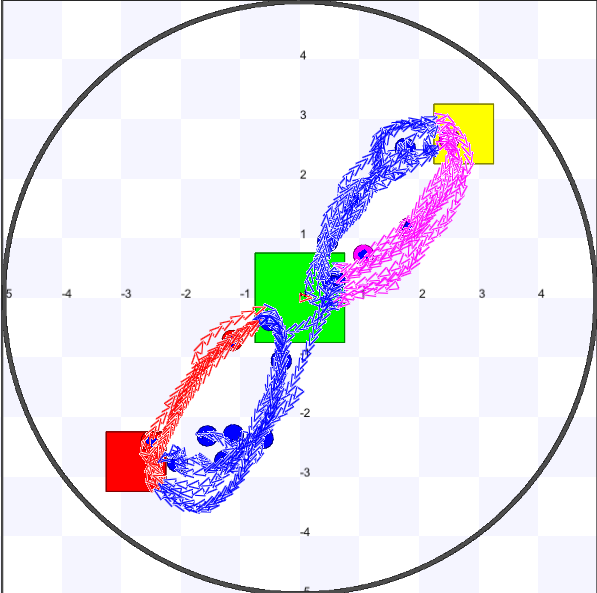
\includegraphics[width=0.49\linewidth]{embodied.png}
   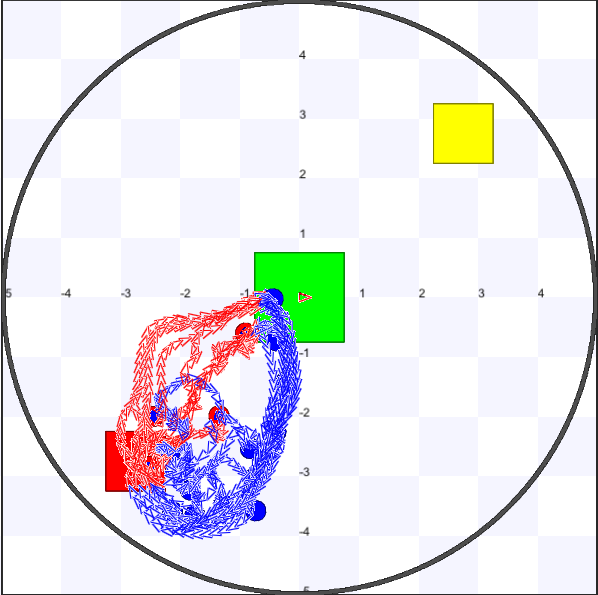
\includegraphics[width=0.49\linewidth]{SO_LOST.png}
   \centering
   \caption{Trails formed in an empty environment using our embodied apprach outlined in section \ref{sec:embodied_approach} (left) and SO-LOST (right)}
   \label{fig:grid_visualization}
\end{figure}

\section{RELATED WORKS}
Various works of ant-inspired trail following algorithms have been published, ranging from leaving real chemical trails \cite{Rus-
sell et al. (1994)} to infra-red message transmission \cite{Payton et al. (2001)}. 

Our work closely follows from Localization-Space Trails (LOST) \cite{LOST} and its variants which is suitable for imperfectly localized robots. A brief review of LOST will be provided in subsection \ref{ssection:LOST_review}. The method is to generate and share short-lived waypoints (\emph{crumbs)} by robots, which contain some information (estimated distance to target, time to target, density of waypoints, to-source or to-sink label). By following these crumbs, robots can find optimal path between source and home. In the Spread-Out LOST (SO-LOST) which is a modified version of LOST, it tries to increase the scalability by minimizing mutual spatial inference between robots which is done by shifting crumbs in a trail from source to home and home to source for a single source, single sink. 

the Multi-Objective LOST (MO-LOST) tries to reduce mutual spatial inference for paths with multiple sources, multiple sinks by shifting the crumbs of a trail which is crossing other crumbs of the other trails. In the Blinkered LOST (Blinkered LOST) it tries to modulate the field of the view (FOV) of the robots' trail-detecting sensor. it shows that the global throughput is a function of robot FOV, means that with narrower FOVs, it performs better in large populations, since narrrower FOV causes multiple trails to be maintained, so that the system can support larger population sizes before saturating due to inference.

\subsection{LOCALIZATION-SPACE TRAILS REVIEW} \label{ssection:LOST_review}

\begin{figure}
   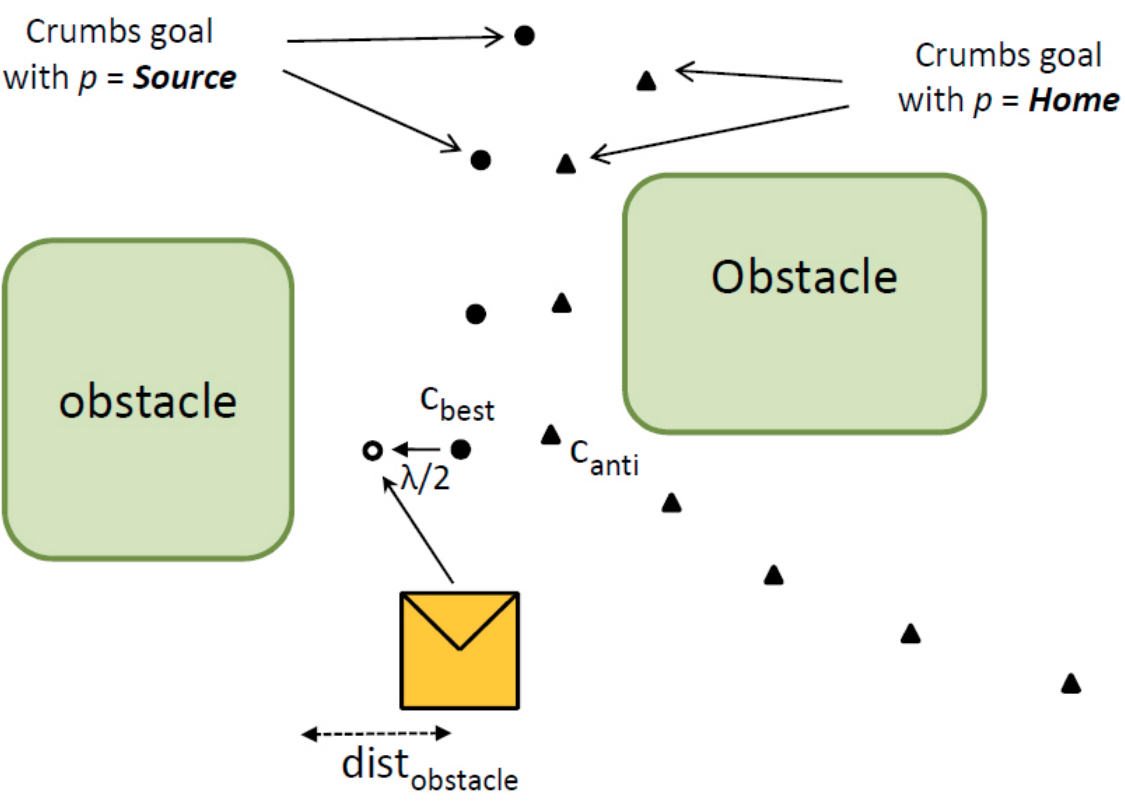
\includegraphics[width=0.9\linewidth]{SO_LOST_crumb_laying.png}
   \centering
   \caption{Trail laying behavior in SO-LOST. The robot is following trail to source (filled circle) and changes its direction to new point (empty circle) to keep distance from trail leading to home (triangles).}
   \label{fig:SO_LOST_crumbnexist_laying}
\end{figure}

LOST generates trails between the locations of \emph{Events} which in our case is reaching source and reaching home. When an Event occurs to robot, its pose in localization space is recorded as \emph{Place} represented by tuple $[Event, Pose]$. Other robots can interpret the coordinates of a place in their own frame of reference. To guide robots between these Events, waypoints called \emph{Crumbs} are laid in every $S$ seconds. A Crumb is a four-tuple $[P_c, L_c, d_c, D_c, t_c]$ containing Place name $P_c$ of place of interest, Localization-space pose $L_c$, estimated distance (in some distance function) between $P_c$ and $L_c$, and $t_c$ the Crumb creation time. A series of Crumbs that lead to the place $P_c$ is referred to as a $Trail$. A robot broadcasts its Trail when an even occurs to it (i.e. when it reaches source or home). All trails are periodically scanned and Crumbs with timestamp older than age threshold $a$ seconds are discarded. This is analogous to ant's pheromone trails evaporating over time.

A robot follows trail to a destination place $P_g$ by heading towards the best crumb $C_L$ within its \emph{field of view}, i.e. within radius $d_f$ of its current position. We use the modified version of this algorithm SO-LOST which lays crumbs certain distance $\lambda$ away from crumbs leading to a different place. Figure \ref{fig:SO_LOST_crumb_laying} shows the crumb laying behavior of the SO-LOST algorithm. 

\section{CONTRIBUTION}

The main contribution of this paper is modification of LOST algorithm to have a simultaneous task allocation which performs better in multiple-source, single-home setting in both large and small population sizes. Two approaches were explored:

\begin{enumerate}
  \item Embodied approach: Subtle modification to LOST using trail density as a proxy for congestion which has the emergent effect of maintaining multiple trails leading to different sources
  \item Explicit allocation approach: Allocate robots to different sources with a goal of uniform distribution of robots along different trails (with consideration of the distances of the sources).
\end{enumerate}

In the following sections, we will describe these approaches with quantitave evaluations.

\section{EMBODIED APPROACH} \label{sec:embodied_approach}
% what is the reason LOST fails, and how did you mitigate it
% Implementation details

\begin{figure}
   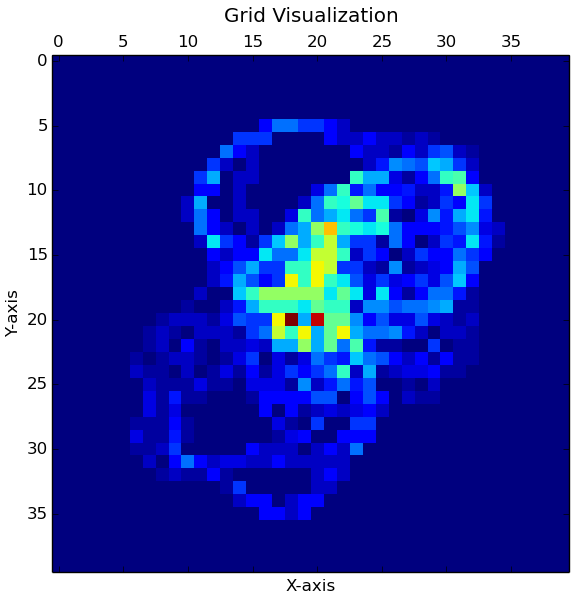
\includegraphics[width=0.49\linewidth]{grid1.png}
   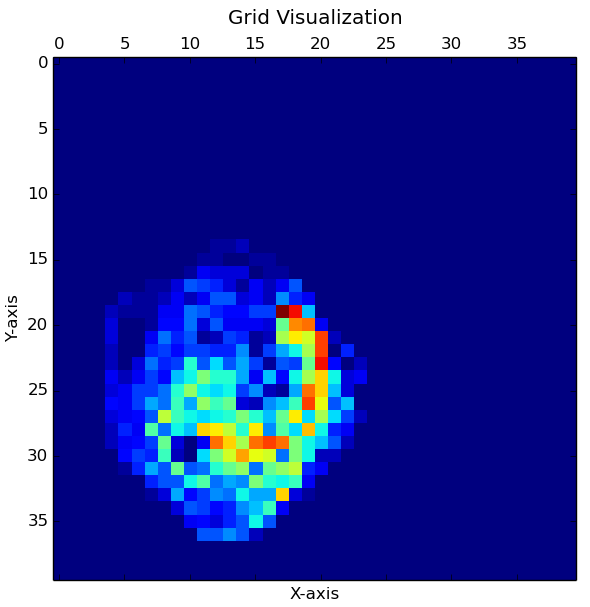
\includegraphics[width=0.49\linewidth]{grid2.png}
   \centering
   \caption{Grid visualization in embodies approach (left) and original version of SO-LOST (right). The home is at center while the sources are at top-right and bottom-left}
   \label{fig:grid_visualization}
\end{figure}

This approach maintains trails to multiple sources without keeping track of the number of sources discovered so far. The general workings of this approach is same as that of LOST algorithm where the robots try to follow the best crumb in their immediate neighbourhood. The crumbs are not labelled with source identification and the robots still make local decision without explicitly considering the multiple sources available. 

The reason LOST and its other variants converge to a single congested trail is that the robots try to minimize the distance to the trail without considering the congestion in the trail. Even when time to target is using as distance metric instead of physical distance, the final trail is still congested for large population sizes. 

This conflict here is whether to follow the shortest path discovered so far or avoid following congested trail which potentially leading to the target with shortest distance. To make a better decision, we take both these factors into account and make decision based on both factors. For this, the distance function is formulated as follows:

\begin{equation}
\begin{split}
   d = w_{time\_to\_target}  \cdot time\_to\_target + \\
          w_{crumb\_density} \cdot crumb\_density
\end{split}
\end{equation}

where $time\_to\_target$ is the time to target encoded in the crumbs and $crumb\_density$ local density of trail around a crumb (to be discussed shortly).

The best values of $w_{time\_to\_target}$ and $w_{crumb\_density}$ were found to be  $0.3$ and $0.7$ respectively from experiments\footnote{The scaling of the weights does not affect the performance. So experiments were done with weights that summed to one}. Note that when $w_{crumb\_density}$ is set to $0$, the algorithm is the same as SO-LOST.

This method not only maintains trails leading to multiple sources, each trail isn't just a single curve of crumbs (Figure \ref{fig:grid_visualization}). Hence, there are multiple side trails that lead to the same source.

\begin{algorithm}
\caption{Embodied Approach}\label{algorithm:1}
\begin{algorithmic}
\Procedure{DIST(c)}{}
  \State $\bold{return} \text{ } w_{d_c} \cdot c.d_c + w_{density} \cdot c.density$
\EndProcedure
\BState
\State $\Theta = \text{all the crumbs in the robot's FOV}$
\State $\Sigma =\{ c | c \in \Theta \text{ } \Lambda \text{ } (c. p_c = robot.goal) \}$
\State $\Pi =\{ c | c \in \Theta \text{ } \Lambda \text{ } (c.p_c \neq robot.goal) \}$
\\
\State $\lambda = Min(crumb\_avoid, \text{ } dist\_obstacle)$
\\
\State $c_{best} = c \text{ s.t. } (c \in \Sigma) \text{ } \Lambda \text{ } (\nexists c' \in \Sigma \text{ s.t. } DIST(c) > DIST(c'))$

\\
\If {$(\exists c_{anti} \in \Pi \text{ s.t. } dist(c_{anti}, robot) < crumb\_avoid) $}
  \State $\text{Shift direction } \lambda \text{ orthogonal to current trail}$
\Else
   \State $\text{Follow the } c_{best}$
\EndIf

\end{algorithmic}
\end{algorithm}

\subsection{CRUMB DENSITY IMPLEMENTATION}
% 2D histogram of crumbs
% world divided to 2D grids. Each cell contains number of crumbs within it
% algorithm: whenever a crumb is created, increment corresponding cell in the grid. when a crumb is destroyed, decrease the corresponding cell
% the size of cell chosen 0.25 m (talk about effects of changing this?)

For finding crumb density, we implemented an additional data structure which is a 2D grid that spans the simulation world. Each cell of the grid contains the number of crumbs within it. Hence, the grid represent a histogram of crumbs. The $crumb\_density$ around a crumb is then the number of crumbs in the cell it belongs to divided by total number of crumbs present. We used cells of size $0.25$ x $ 0.25$  m. This is approximation of a robot's size. Figure \ref{fig:grid_visualization} shows a visualization of our grid data structure. A brighter value means higher number of crumbs. The fact that SO-LOST implementation converges to a single source is clearly visible while our approach maintains trails leading to both the sources.

\subsection{DRAWBACKS OF THIS APPROACH} \label{ssec:drawbacks_of_1}
% a lot of parameters, need to set it manually
% paradox: avoiding congested trail and exploiting the nearest source
% no guarantee of convergence to multiple sources: if by chance all the robots discover the same source, they stick with it. Redeeming factor: with large population size, they tend to find multiple sources

A major drawbacks of this approach is that there are a lot of parameters that needed to be handtuned. These parameters are evaporation rate of crumbs, grid size and weights of density and time to target in distance function. Even though we were able to get moderate invariance to size of the world, number of robots, number of sources and distances of the sources, these parameters still need fine tuning when used in drastically different setting.

A future extension would be to change these parameters dynamically. For example, we can set evaporation rate based on distance between source and home such that multiple cycles on the same trail does not give a false impression of congestion. We would also like to note that the need to finetune the evaporation rate on different distances between source and home is not inherent to our approach and almost all ant-trail based algorithms would require this. But  performance our method is particularly sensitive to this parameter.

Also, there is also no guarantee of convergence to multiple sources. If by chance all the robots discover the same source, there will only be a single trail leading to that source (although this is highly unlikely if we have large number of robot).

\section{EXPLICIT ALLOCATION APPROACH} 
% To mitigate the shortcomings of our previous approach
% Instead of using crumb density as a proxy for congestion, keep track of the actual congestion (number of robots current pursuing a source)
% Ensure that the spatial interference between the robots is minimum (allocate robots to source such that there is enough space per robot)
% Our nice equation

This method was explored to mitigate the shortcomings of our previous approach. Using crumb density as a heuristic of congestion introduces unwanted dependence on evaporation rate and trail length as discussed in the previous subsection \ref{ssec:drawbacks_of_1}. This approach, instead of using approximation, utilizes the actual congestion in different trails. It also modifies the crumb data structure to include the source the crumb is leading to and the total euclidean distance from that crumb to the target, so the new crumb data structure with respect to the its definition in the LOST review section is a tuple $C = [P_c, S_c, L_c, d_c, D_c, t_c]$ which contains the name of the Place $P_c$ to which it refers [source or sink], source id that the crumb is leading to $S_c$, a localization space pose $L_c$, an estimate $d_c$ of the distance from $L_c$ to the target $P_c$ which comes from a distance function that assume time as distance in the original version of LOST, an estimate of total euclidean distance from the crumb to the target, and the time $t_c$ containing the creation time of the crumb.

We also maintain a global data structure to keep track of numbers of robot currently following different sources. It is implemented as a hash table with all the discovered sources as its key and the number of robots in trail leading to a source as its value. This structure is updated every time a robot reaches home and is allocated to a source.

When a robot reaches home, it checks congestion in every trail. We formulation our \emph{congestion\_factor} as follows:

\begin{equation}
\begin{split}
  congestion\_factor = \dfrac{(R_{SIZE} + D_{SAFE}) \cdot n_t}{ d_t }
\end{split}
\end{equation}

where $R_{SIZE}$ is the size of robot (diameter) in meters, $D_{SAFE}$ is a safe distance (meters) we need to maintain between the robots, $n_t$ is the number of robots currently in that trail and $d_t$ is the length of the trail (meters)

The ideal $congestion\_factor$ is $1$ where the robots form a tight loop in the trail with a safety distance  $D_{SAFE}$ between each other. Whenever a robot reaches home, it calculates $congestion\_factor$ for each source and decides to choose the source with minimum $congestion\_factor$ that is less than $1$. If no trail is available that has $congestion\_factor$ less than 1, the robot decides not to follow any trail and move randomly to find other food sources. After choosing the source (or deciding to explore randomly), the hash table is updated if needed.

Although this method maintains trail leading to multiple sources and increases our throughput, but in the case of having paths that are almost equally congested, robots can switch back and forth between sources. We introduce an \emph{inertia} factor for convergence of robots to a particular source; a robot decides to switch from one source to another only if the $congestion\_factor$ is better than that of previous source by a fixed threshold.

This approach will have a better performance even in single source setting as the trail between source and home is maintained such that there is minimum change of interference between the robots. Experimental results showing this will be provided in the following section. 

In our implementation, we do not restrict the wandering robots that were not assigned to any known source to cross existing trails. A better performance will likely be achieved by having such restrictions.

\begin{algorithm}
\caption{Explicit Allocation Approach}\label{algorithm:2}
\begin{algorithmic}
\State $\text{\# Congestion factor of a source } s$
\Procedure{$C_f(s)$}{}
  \State $\Sigma = \text{all the crumbs}$
  \State $c_{farthest} =  c \text{ s.t. } (c \in \Sigma) \text{ } \Lambda \ (c.Sc=s) \text{ } \Lambda$
  \State  $\text{                                                 }(\nexists c' { s.t. } dist(c', home) < dist(c, home))$
  \\
  \State $\bold{return} \text{ } \dfrac{(R_{SIZE} + D_{SAFE})  s.num\_robots}{ c_{farthest}.d_t }$
\EndProcedure
\State $\Theta = \text{Known sources}$
\State $s_{prev} = \text{previous source the robot was following}$
\State $s_{best} = s \text{ s.t. } (s \in \Theta) \text{ } \Lambda \text{ } (\nexists s' \in \Theta \text{ s.t. } C_f(s') < C_f(s))$

\\
\If {$(s \neq \phi) $}
  \If {$(C_f(s_{best}) - C_f(s_{prev}) < threshold)$}
     \State $s_{chosen} = s_{best}$
  \Else
     \State $s_{chosen} = s_{previous}$
  \EndIf
\Else
   \State $\text{Random move}$
\EndIf

\end{algorithmic}
\end{algorithm}

\subsection{POSSIBLE MODIFICATIONS FOR DISTRIBUTEDNESS}
% one robot decides to stay home doing the book-keeping and allocates robots to different source 
% robots communicate with each other and update information of the number of robots in different trails
In the previous section we mentioned a new data structure that used to keep number of robots in each path, which makes this approach centralized, the following defintion of crumbs is suggested: $C = [P_c, S_c, L_c, d_c, D_c, t_c, R_{UDID}]$ in which we have a new information containing a random constant unique identity for each robot that is generated when they start working, in this case, instead of having a hash table which stores the number of robots in each path, each robot can read crumbs and see how many unique identity are in this path. However, persistence of the crumbs still depend on the evaporation rate and the length of the trail. In order to solve this issue, since the path converges after a while, each robot knows an estimate of traveling time, so they can count the number of robots based on the crumbs where the creation timestamp is greater than the average traveling time.

Another way of making this approach distributed is having an agent at home which is incharge of maintaining the hash table and relays the information when a robot reaches home, based on which the robot decides the source to pursue. For this, we can either place a server like setup near home or arbitrarily have one of the robots stay at home to assume the role of conductor.

\section{EXPERIMENTS} \label{section:experiments}

\subsection{SIMULATION SETUP}

We used Stage simulator \cite{STAGE} to implement SO-LOST, Embodied Approach and Explicit Allocation Approach. We tested in the empty world of size 10x10. Stage's Irobot Roomba robots were used with SICK LMS200 laser rangefinder. The middle green square is the home, the red square is source 1, the blue square is source 2 and the yellow square is source 3. Red robots are carrying resources from source 1, magenta robots are carrying resources from source 2 and the cyan robots are carrying resources from source 3. Robots that are not carrying any resource are colored blue. Each trial was run for 10 minutes and the total number of resources delivered at the end of the trial is our performance metric. Due to stochastic nature of all the methods, we run 5 trials for each setting.

The experiments we conducted used the following parameter settings:

\begin{table}[ht]                                                              
  \begin{center}
  % \scalebox{0.9}{
    \begin{tabular}{|c|c|c|c|}                                                
    \hline
      Parameter & Embodied & Explicit & SO-LOST\\                                  
    \hline                                                                    
      $Evaporation\ rate$ & 10Hz & 10Hz & 10Hz\\ % evaporation rate
    \hline
      $d_f$ & 1.5m & 1.5m & 1.5m\\ % trail detector sensor range              
    \hline
      $S$ & .2s & .2s & .2s\\ % frequency of dropping a crumb on the map    
    \hline
      $Minimum\ Trail\ Distance$ & 0.75m & 0.75m & 0.75m\\ % expected distance between trails in SO-LOST      
    \hline
      $Grid\ Cell\ Size$ & 0.25 & N/A & N/A\\ % Cell size in Grid (embodied approach)      
    \hline
      $W_{crumb\_density}$ & 0.7 & N/A & 0.0\\ % weight corresponding to density            
    \hline
      $W_{time\_to\_target}$ & 0.3 & N/A & 1.0\\ % weight corresponding to distance            
    \hline
      $Inertia\ Factor$ & N/A & 0.3 & N/A\\ % inertia factor (explicit approach)          
    \hline
      $Max\ Congestion\ Factor$ & N/A & 1.2 & N/A\\ % congestion factor (explicit approach)        
    \hline
    \end{tabular}
   \caption{Parameters Settings for Experiments}                                
    \label{table:parameter_settings}
  \end{center}
\end{table}

\subsection{RESULTS}

\begin{figure}[h]
  \begin{subfigure}{.25\textwidth}
      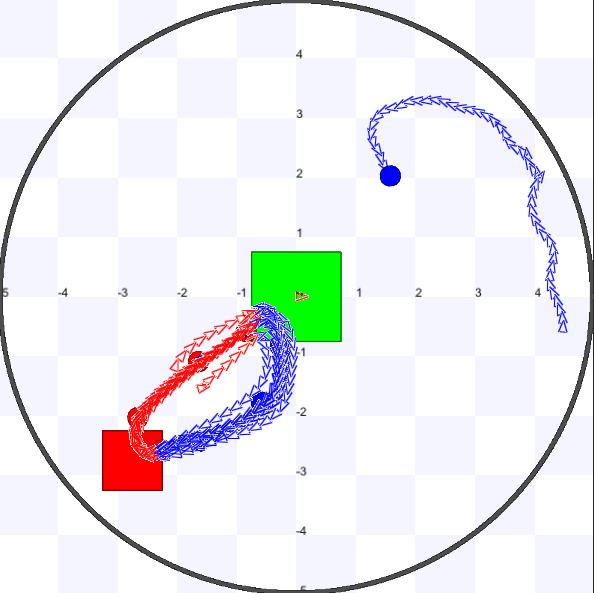
\includegraphics[width=0.9\linewidth]{images/explicit/1/raw/8.png}
         \centering
         \caption{Explicit Approach}
   \end{subfigure}%
     \begin{subfigure}{.25\textwidth}
       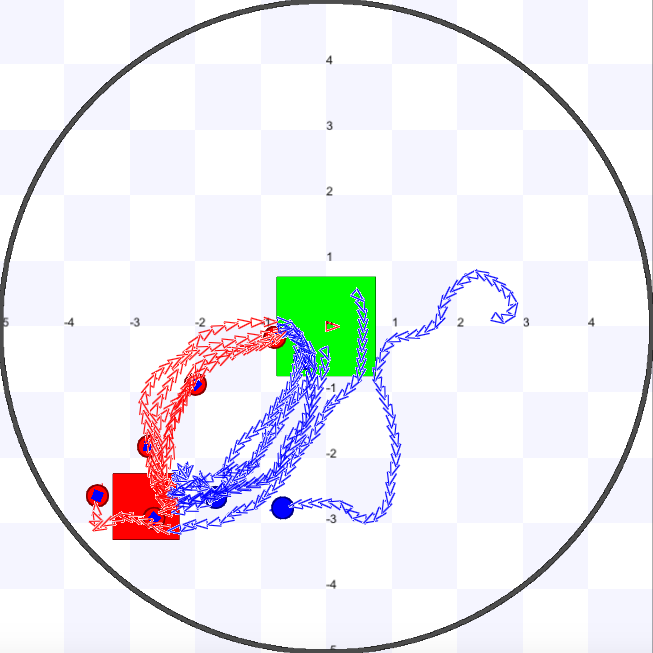
\includegraphics[width=0.9\linewidth]{images/embodied/1/raw/8.png}
          \centering
          \caption{Embodied Approach}
     \end{subfigure}
    \centering
     \begin{subfigure}{.25\textwidth}
       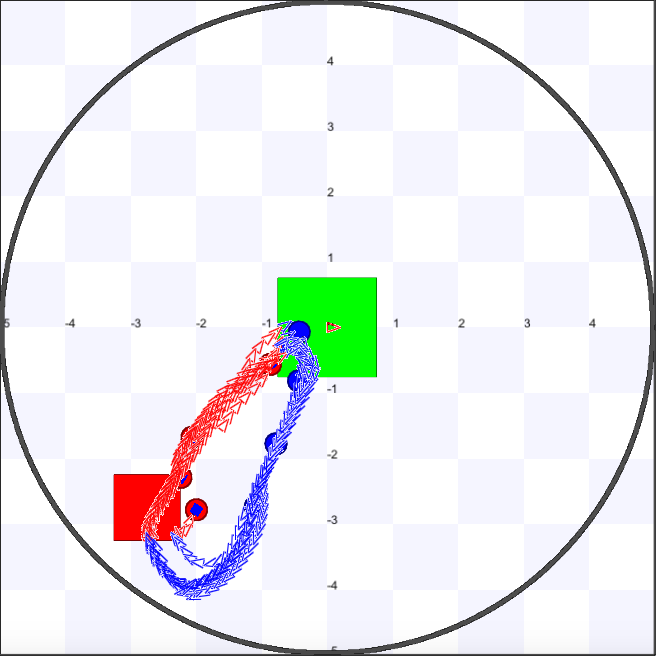
\includegraphics[width=0.9\linewidth]{images/so-lost/1/raw/8.png}
          \centering
          \caption{SO-LOST}
     \end{subfigure}
   
   \centering
   \caption{Screenshot after 10 minutes of simulation time: single source, 8 robots}
   \label{fig:screenshot_1_source}
\end{figure}

\begin{figure}[h]
  \begin{subfigure}{.25\textwidth}
      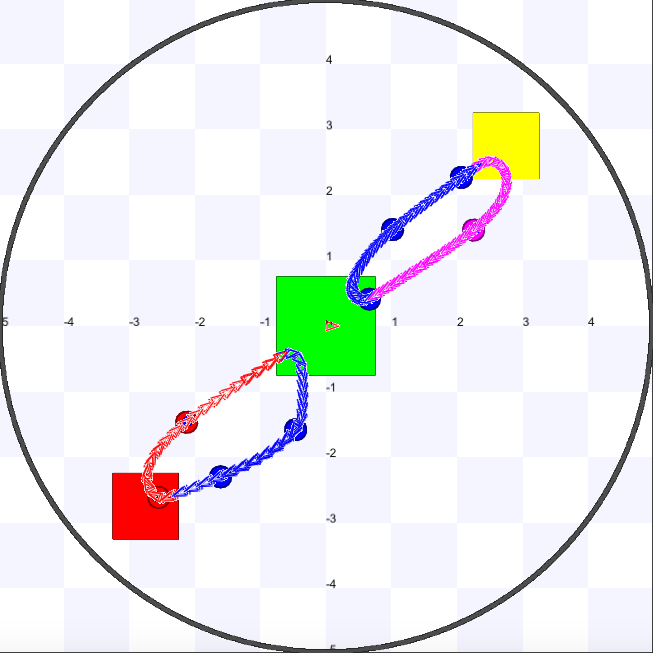
\includegraphics[width=0.9\linewidth]{images/explicit/2/raw/8.png}
         \centering
         \caption{Explicit Approach}
   \end{subfigure}%
     \begin{subfigure}{.25\textwidth}
       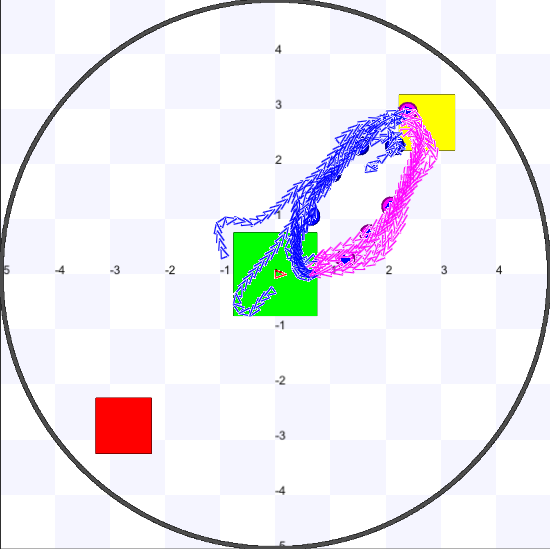
\includegraphics[width=0.9\linewidth]{images/embodied/2/raw/8.png}
          \centering
          \caption{Embodied Approach}
     \end{subfigure}
    \centering
     \begin{subfigure}{.25\textwidth}
       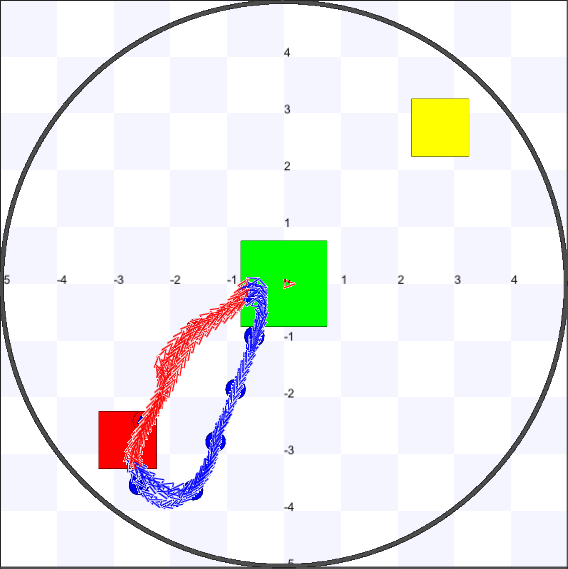
\includegraphics[width=0.9\linewidth]{images/so-lost/2/raw/8.png}
          \centering
          \caption{SO-LOST}
     \end{subfigure}
   
   \centering
   \caption{Screenshot after 10 minutes of simulation time: 2 sources, 8 robots}
   \label{fig:screenshot_2_source}
\end{figure}

\begin{figure}[h]
  \begin{subfigure}{.25\textwidth}
      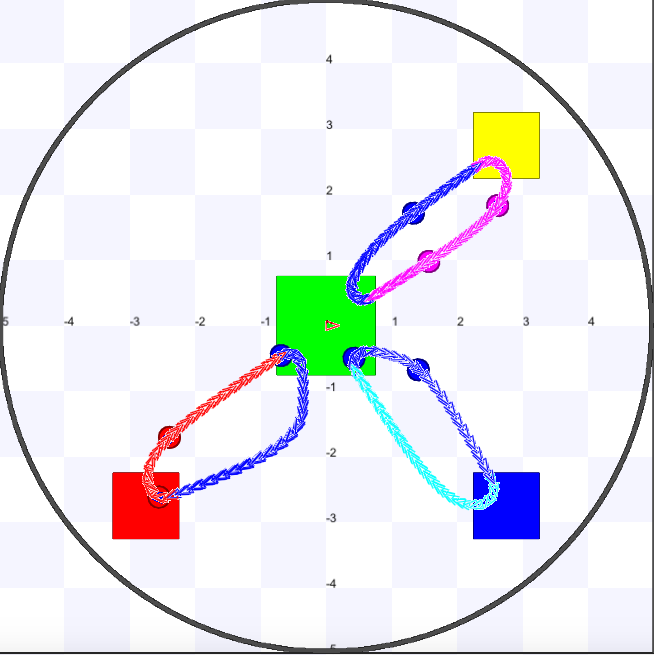
\includegraphics[width=0.9\linewidth]{images/explicit/3/raw/8.png}
         \centering
         \caption{Explicit Approach}
   \end{subfigure}%
     \begin{subfigure}{.25\textwidth}
       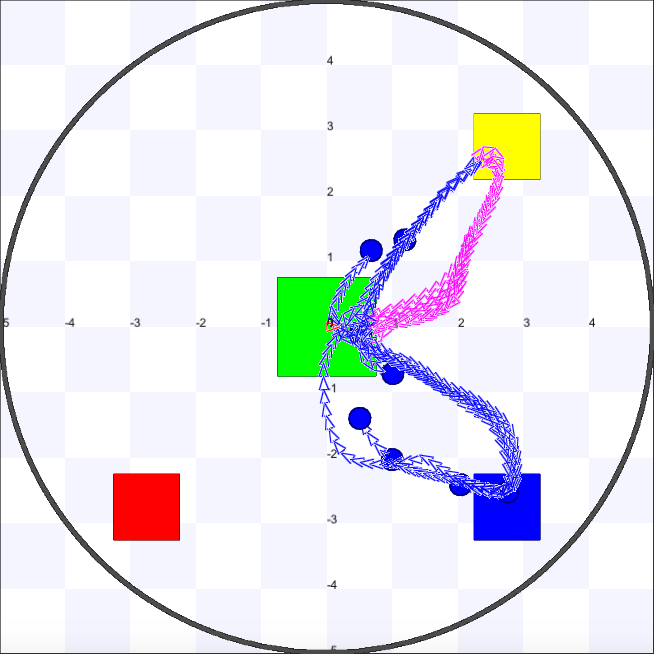
\includegraphics[width=0.9\linewidth]{images/embodied/3/raw/8.png}
          \centering
          \caption{Embodied Approach}
     \end{subfigure}
    \centering
     \begin{subfigure}{.25\textwidth}
       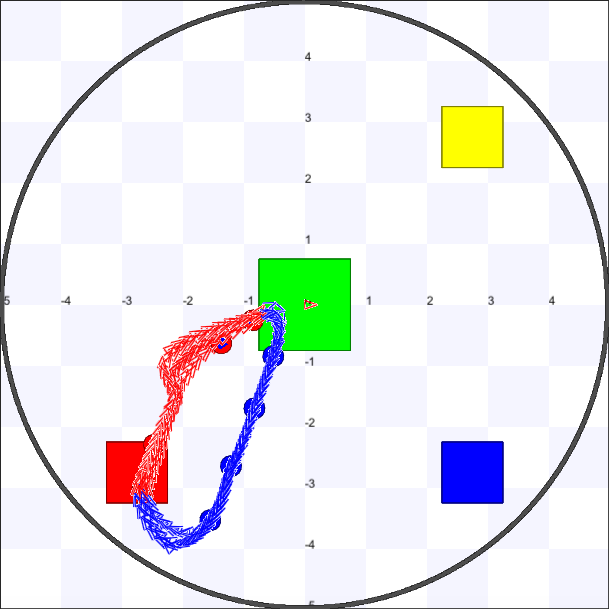
\includegraphics[width=0.9\linewidth]{images/so-lost/3/raw/8.png}
          \centering
          \caption{SO-LOST}
     \end{subfigure}
   
   \centering
   \caption{Screenshot after 10 minutes of simulation time: 3 sources, 8 robots}
   \label{fig:screenshot_3_source}
\end{figure}

\subsection{DISCUSSION}
% increasing the number of robots, more robots won't be assigned to any source and left to wander. But these wandering robots interfere with the robots in existing trails and degrade the performance. 

% The first approach is highly dependent on number of parameters. It has high variance when number of robots large

% 12 robots, 3 sources: In some cases the robots can't find the third source for a longer time. 

\section{CONCLUSIONS AND FUTURE WORKS}

In this paper, we outlined two approaches for improving LOST algorithm for better throughput in a multiple-source, single-home setting. We have provided experimental results showing improved performance compared to a variant of LOST (SO-LOST) both quantitavely and qualititavely.  The robots take into account the congestion in the trails either explicitly or implicitly to make better decisions regarding which trail to follow. 

In our future works we will implement a fully distributed version of our algorithm, potentially with real robots. Another extension can be implementing Maximum Sustainable Yield (MSY) \cite{MSY_PAPER Hjort et al. 1933 } where the sources have a finite (and possibly different) resource growth rate. Previous works in multi-robot MSY foraging \cite{Song and Vaughan 2013} and \cite{Zhang and Zhao Song 2016} rely on known source position. We can extend our current work to deal with simultaneous source finding and MSY in multiple-souce, single-home setting. 

We will also improve our navigation strategies. There are lot of room for improvement in our obstacle avoidance and trail-following behavior which could lead to better performance. 

\addtolength{\textheight}{-12cm}   % This command serves to balance the column lengths
                                  % on the last page of the document manually. It shortens
                                  % the textheight of the last page by a suitable amount.
                                  % This command does not take effect until the next page
                                  % so it should come on the page before the last. Make
                                  % sure that you do not shorten the textheight too much.

%%%%%%%%%%%%%%%%%%%%%%%%%%%%%%%%%%%%%%%%%%%%%%%%%%%%%%%%%%%%%%%%%%%%%%%%%%%%%%%%



%%%%%%%%%%%%%%%%%%%%%%%%%%%%%%%%%%%%%%%%%%%%%%%%%%%%%%%%%%%%%%%%%%%%%%%%%%%%%%%%



%%%%%%%%%%%%%%%%%%%%%%%%%%%%%%%%%%%%%%%%%%%%%%%%%%%%%%%%%%%%%%%%%%%%%%%%%%%%%%%%
\section*{APPENDIX}

Appendixes should appear before the acknowledgment.

\section*{ACKNOWLEDGMENT}

The preferred spelling of the word �acknowledgment� in America is without an �e� after the �g�. Avoid the stilted expression, �One of us (R. B. G.) thanks . . .�  Instead, try �R. B. G. thanks�. Put sponsor acknowledgments in the unnumbered footnote on the first page.



%%%%%%%%%%%%%%%%%%%%%%%%%%%%%%%%%%%%%%%%%%%%%%%%%%%%%%%%%%%%%%%%%%%%%%%%%%%%%%%%

References are important to the reader; therefore, each citation must be complete and correct. If at all possible, references should be commonly available publications.

% references section 
\bibliography{root}




\end{document}
